\documentclass[floatfix,aps,prd,nofootinbib,superscriptaddress,preprint]{revtex4}


\pdfoutput=1
\usepackage{graphicx}
\usepackage{amsmath}
\usepackage{amssymb}
\usepackage{slashed}
\usepackage{mathtools}
\usepackage[utf8]{inputenc}
\usepackage[colorlinks=true,linkcolor=blue,bookmarksopen,bookmarksnumbered]{hyperref}
\usepackage{color}
\usepackage[usenames,dvipsnames]{xcolor}
\usepackage[normalem]{ulem}
\usepackage{soul}
\usepackage{units}
\usepackage{rotating}
\usepackage{hhline,multirow,tabularx}
\usepackage{bm}
\usepackage{hyperref}
\usepackage[compatibility=false]{caption}
\usepackage{subcaption}
\usepackage{mdframed}

% paths
\newcommand*{\FigPath}{./figures}%

% math macros 
\newcommand{\T}[1]{\boldsymbol{#1}_{\text{T}}}
\newcommand{\kT}{\ensuremath{k_{\rm T}}}
\newcommand{\ktmax}{\ensuremath{k_{\rm T max}}}
\newcommand{\ktmaxsq}{\ensuremath{k_{\rm T max}^2}}
\newcommand\3[1]{\boldsymbol{#1}}
\newcommand{\Tsc}[2]{#1_{#2\text{T}}}
\newcommand{\Tscsq}[2]{#1^2_{#2\text{T}}}
\newcommand{\no}{\nonumber \\}
\newcommand{\parz}[1]{\ensuremath{\left(#1\right)}}
\newcommand{\order}[1]{\ensuremath{O\parz{#1}}}
\newcommand{\mhad}{\ensuremath{M}}
\newcommand{\alfa}{\ensuremath{\alpha}}
\newcommand{\xbj}{\ensuremath{x_{\rm bj}}}
\newcommand{\xn}{\ensuremath{x_{\rm n}}}
\newcommand{\mquark}{\ensuremath{m_{q}}}
\newcommand{\mgluon}{\ensuremath{m_{s}}}
\newcommand{\spectator}{\ensuremath{p_s}}
\newcommand{\jet}{\ensuremath{p_q}}
\newcommand{\pdfblob}{{\ensuremath{\mathcal F}}}
\newcommand{\ffblob}{{\ensuremath{\mathcal J}}}
\newcommand{\prop}{{[ \ensuremath{\rm Prop} ]}}
\newcommand{\num}{{\ensuremath{\rm T}}}
\newcommand{\jac}[1]{{\ensuremath{[ {\rm Jac_{#1}} ] }}}
\newcommand{\arrowcom}[1]{\textcolor{red}{\textbf{$\Longrightarrow$ #1}} \\}
\newcommand{\arrowcomtwo}[1]{\textcolor{blue}{ \textbf{$\Longrightarrow$ #1}} \\}
\newcommand{\arrowcomthree}[1]{\textcolor{magenta}{ \textbf{$\Longrightarrow$ #1}} \\}
\newcommand{\diff}[1]{\mathrm{d}#1}
\newcommand{\moderate}{{\color{red}low}}

\newcommand{\vect}[1]{\ensuremath{{\bm{#1}}}}
\newcommand{\bfkperp}{{\bf k}_\perp} 
\newcommand{\bfpperp}{{\bf P}_\perp} 
\newcommand{\bfhp}{\hat{\bf h}} 
\newcommand{\bfPhperp}{{\bf P}_{hT}}
\newcommand{\Phperp}{P_{hT}}
\newcommand{\kperp}{k_\perp}
\newcommand{\pperp}{P_\perp}
\newcommand{\avkperp}{\la \kperp^2 \ra}
\newcommand{\avpperp}{\la \pperp^2 \ra}
\newcommand{\la}{\langle}
\newcommand{\ra}{\rangle}

\newcommand{\bt}{b_{\rm T}}
\newcommand{\qt}{q_{\rm T}}


% ref macros
\newcommand{\eref}[1]{Eq.~(\ref{e.#1})}
\newcommand{\erefs}[2]{Eqs.~(\ref{e.#1})--(\ref{e.#2})}
\newcommand{\fref}[1]{Fig.~\ref{f.#1}}
\newcommand{\frefs}[2]{Figs.~\ref{f.#1}--\ref{f.#2}}
\newcommand{\aref}[1]{Appendix~\ref{a.#1}}
\newcommand{\sref}[1]{Sec.~\ref{s.#1}}
\newcommand{\ssref}[1]{Section~\ref{ss.#1}}
\newcommand{\sssref}[1]{Section~\ref{sss.#1}}
\newcommand{\tref}[1]{Table~\ref{t.#1}}

\begin{document}
	
\title{Energy Evolution of Delta Function for Jet Physics}
	
\author{Andrew Gordeev}
\email{agordeev@ucla.edu}
\affiliation{Department of Physics and Astronomy, University of
	California, Los Angeles, CA 90095, USA}

\author{Zhong-Bo Kang}
\email{zkang@physics.ucla.edu}
\affiliation{Department of Physics and Astronomy, University of
California, Los Angeles, CA 90095, USA}

\author{John D. Terry}
\email{johndterry@physics.ucla.edu}
\affiliation{Department of Physics and Astronomy, University of
California, Los Angeles, CA 90095, USA}
	
\begin{abstract}
	Blank for now
\end{abstract}
	
\maketitle
	
%%%%%%%%%%%%%%%%%%%%%%%%%%%%%%%%%%%%

\section{Derivations}

Professor Kang gives us that the energy evolution of $J$ is given by

\begin{align}
	\frac{\partial}{\partial ln \mu^2} J(z, \mu) = \frac{\alpha_s(\mu)}{2\pi}\int_z^1 \frac{dx}{x}P(x)J(\frac{z}{x}, \mu).
	\label{e.evo}
\end{align}
Where 
\begin{align}
	P(x) = C_F[\frac{1+x^2}{(1-x)_+}+\frac{3}{2}\delta(1-x)]
	\label{e.frag}
	\qquad
	\int_0^1 dx \frac{f(x)}{(1-x)_+} = \int_0^1 dx \frac{f(x)-f(1)}{(1-x)}
\end{align}

Plugging $\eref{frag}$ in $\eref{evo}$ we obtain

\begin{align*}
\frac{\partial}{\partial ln \mu^2} J(z, \mu) = \frac{\alpha_s(\mu)}{2\pi}\int_z^1 \frac{dx}{x}C_F[\frac{1+x^2}{(1-x)_+}+\frac{3}{2}\delta(1-x)]J(\frac{z}{x}, \mu).
\end{align*}

Following the chain rule, 

\begin{align}
	\frac{\partial}{\partial \mu} J(z, \mu) &= \frac{\partial}{\partial ln \mu^2} J(z, \mu) \cdot \frac{\partial ln \mu^2}{\partial \mu} \nonumber \\
	&= \frac{\alpha_s(\mu)}{\pi\mu}\int_z^1 \frac{dx}{x}C_F \Big[\frac{1+x^2}{(1-x)_+}+\frac{3}{2}\delta(1-x) \Big] J(\frac{z}{x}, \mu) \nonumber \\
	&= \frac{\alpha_s(\mu) C_F}{\pi\mu}\int_z^1 \frac{dx}{x}\frac{1+x^2}{(1-x)_+}J(\frac{z}{x}, \mu) + \frac{3\alpha_s(\mu) C_F}{2 \pi\mu}\int_z^1 \frac{dx}{x} \delta(1-x)J(\frac{z}{x}, \mu)
    \label{e.split}
\end{align}

To evaluate the left integral in $\eref{split}$, we use the fact that

\begin{align*}
	\int_z^1 dx \frac{f(x)}{(1-x)_+} &= \int_0^1 dx \frac{f(x)}{(1-x)_+} - \int_0^z dx \frac{f(x)}{(1-x)_+} \\
	&= \int_0^1 dx \frac{f(x)-f(1)}{(1-x)} - \int_0^z dx \frac{f(x)}{(1-x)} \\
	&= \int_z^1 dx \frac{f(x)-f(1)}{(1-x)} + \int_0^z dx \frac{f(x)}{(1-x)} - \int_0^z dx \frac{f(1)}{(1-x)} - \int_0^z dx \frac{f(x)}{(1-x)} \\
	&= \int_z^1 dx \frac{f(x)-f(1)}{(1-x)} + f(1) \cdot ln (1-z).
\end{align*}

Thus,

\begin{align}
	\int_z^1 \frac{dx}{x}\frac{1+x^2}{(1-x)_+}J(\frac{z}{x}, \mu) &= \int_z^1 dx \frac{\frac{1+x^2}{x}J(\frac{z}{x}, \mu) - 2J(z, \mu)}{1-x} + 2J(z,\mu) \cdot ln (1-z).
    \label{e.leftint}
\end{align}

We evaluate the right integral in $\eref{split}$ using the delta function:

\begin{align}
	\int_z^1 \frac{dx}{x} \delta(1-x)J(\frac{z}{x}, \mu) = \frac{1}{2} \cdot \frac{1}{x} J(\frac{z}{x}, \mu)|_{x = 1} = \frac{1}{2}J(z, \mu)
    \label{e.rightint}
\end{align}

Using $\eref{leftint}$ and $\eref{rightint}$, $\eref{split}$ becomes

\begin{align}
	\frac{\partial}{\partial \mu} J(z, \mu) = \frac{\alpha_s(\mu) C_F}{\pi\mu} &\Big( \int_z^1 dx \frac{\frac{1+x^2}{x}J(\frac{z}{x}, \mu) - 2J(z, \mu)}{1-x} + 2J(z,\mu) \cdot ln (1-z) + \frac{3}{4}J(z, \mu) \Big).
    \label{e.dJdmu}
\end{align}

This equation is solved using the RK4 method, setting the initial value of $J$ as an approximation of the delta function: 

\begin{align*}
	J(z, \mu_0) = \delta(1-z) \approx 
    \begin{cases}
    	\frac{2}{a^2} (z-(1-a)) & \text{if } 1-a \leq z \leq 1 \\
        0 & \text{otherwise}
    \end{cases}
\end{align*}

where $a$ is some small constant. To find intermediate values of $J$ in the Runge-Kutta method, we use the approximation 

\begin{align*}
	J(z, \mu + \delta\mu) \approx J(z, \mu) + \delta\mu \cdot \frac{\partial}{\partial \mu} J(z, \mu)
\end{align*}

where $\frac{\partial}{\partial \mu} J(z, \mu)$ is given by $\eref{dJdmu}$.

\section{Results}

$J$ was evolved from 10 GeV to 100 GeV. Figure $\ref{fig:Jmu1}$ shows the results as functions of $z$ for three values of $\mu$.

\begin{figure}
	\centering
 	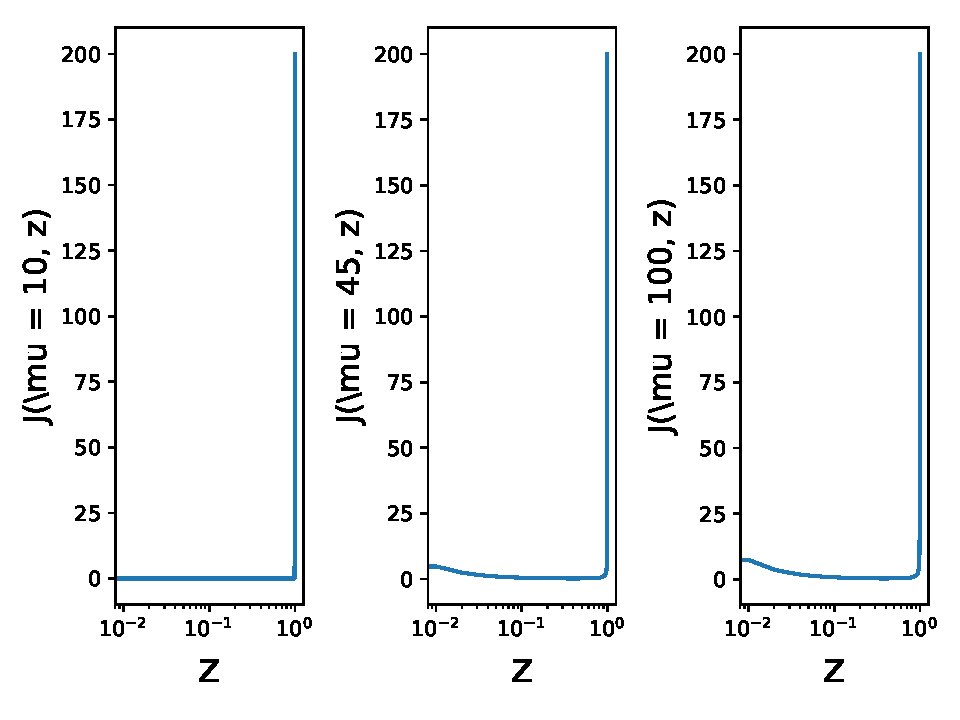
\includegraphics{\FigPath/Jmu1}
  	\caption{Plots of $J$ for initial, intermediate, and final values of $\mu$.}
  	\label{fig:Jmu1}
\end{figure}


\end{document}